\documentclass{beamer}
\usepackage[UTF8]{ctex}
\usepackage{graphicx}
\usepackage{caption}
\usepackage{bookman}
\usetheme{Madrid}
\usepackage{wrapfig}
\graphicspath{ {./texPic/} }
%Information to be included in the title page:
\title{ZooKeeper学习记录}
\author{潘重宇}
\institute{兴业数金}
\date{2022/4/15}

\begin{document}
	
\frame{\titlepage}

\AtBeginSection[]
{
	\begin{frame}
		\frametitle{目录}
		\tableofcontents[currentsection]
	\end{frame}
}

\section{ZooKeeper概念和基础}
\begin{frame}
	\frametitle{ZooKeeper的使命}
	在分布式系统中协作多个任务
\begin{itemize}
	\item<1-> 保障强一致性、有序性和持久性。
	\item<2-> 实现通用的同步原语的能力。
	\item<3-> 简单的并发处理机制。
\end{itemize}
\end{frame}

\begin{frame}
	\frametitle{ZooKeeper架构}
	设计一个用于协作需求的服务的方法往往是提供原语列表,暴露出每个原语的实例化调用方法,并控制这些实例。然而这设计存在一些缺陷:首先我们需要预先提出一份详细的原语列表,或者提供API的扩展,以便引入新的原语;其次,以这种方式实现原语的服务使得应用丧失了灵活性。

\begin{examples}
	分布式锁机制可以说实现了一个重要的原语,同时暴露出创建(create),获取(acquire)和释放(release)三个调用方法。
\end{examples}
\end{frame}

\begin{frame}
	\frametitle{ZooKeeper架构}
	因此,ZooKeeper另辟蹊径,并不直接暴露原语。取而代之,它暴露了由一小部分调用方法组成的类似文件系统的API,以便允许应用实现自己的原语。ZooKeeper操作和维护一个小型的数据节点,这些节点被称为znode,采用类似于文件系统的的层级树进行管理,叶子节点储存了数据信息。
	\begin{figure}[b]
		\caption{ZooKeeper数据树结构示意}
		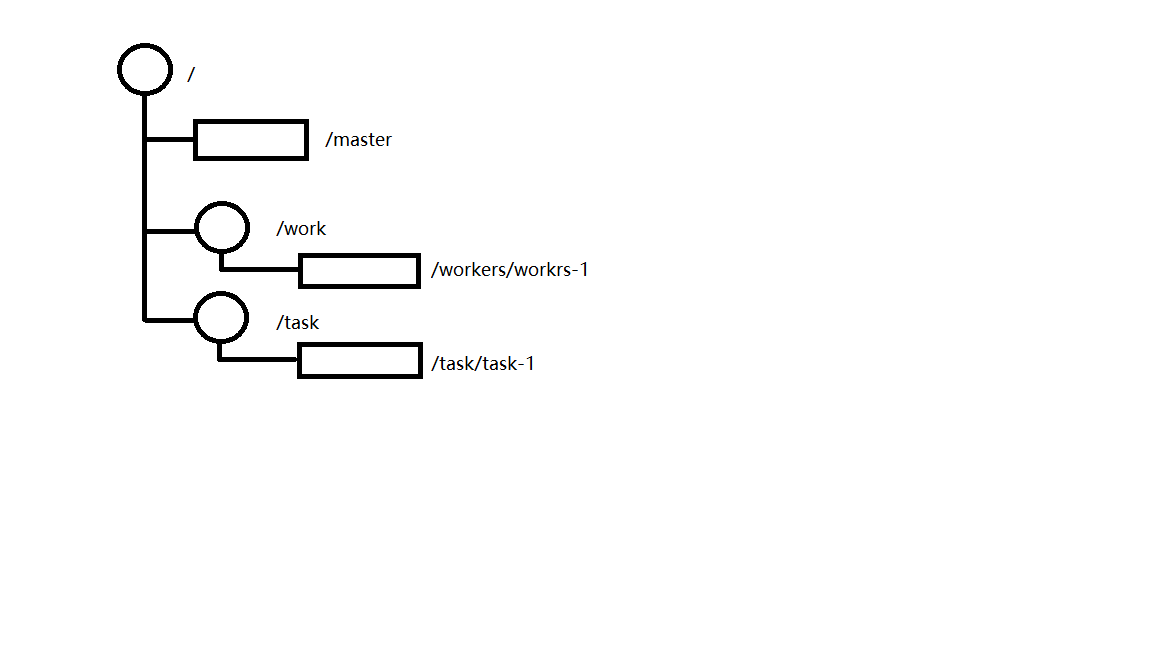
\includegraphics[width=8cm, height=6cm]{zookeper架构.png}
	\end{figure}
\end{frame}

\begin{frame}
	\frametitle{ZooKeeper架构}
	应用通过客户端来对ZooKeeper实现调用,客户端负责与ZooKeeper服务器进行交互。
	\\
	ZooKeeper服务器运行于两种模式下:独立模式(standalone)和仲裁模式(quorum)。独立模式为一个单独的服务器,ZooKeeper状态无法复制。仲裁模式下,具有一组服务器,称其为ZooKeeper集合(ZooKeeper ensemble),它们之间可以进行状态复制,同时服务客户端的请求。
	\\
	在仲裁模式下,ZooKeeper复制集群中的所有服务器的数据树。只要有法定人数的服务器保存了数据,ZooKeeper就可以有效的运行,并且其它的服务器最终也能捕获到数据并保存。
	\begin{block}{法定人数}
		服务器告知客户端安全保存数据前,需要保存客户端数据的服务器的最小个数。法定人数的数量需要保证不管系统延迟或崩溃,服务器主动确认的任何更新请求需要保持下去,直到另一个请求代替它。
	\end{block}
\end{frame}

\begin{frame}
	\frametitle{ZooKeeper架构}
	\begin{block}{法定人数}
		为了避免脑裂现象,法定人数必须大于服务器个数的一半,符合多数原则,并为了更快的相应请求并容忍更多的服务器崩溃,需要确保法定人数足够小。
	\end{block}
	\begin{block}{会话}
		在对ZooKeeper集合执行任何操作前,一个客户端必须先与服务器建立会话。客户端提交给ZooKeeper的所有操作均关联在一个会话上。当一个会话中止时,在这会话期间创建的临时节点将会消失。
		\\
		当客户端通过某特定语言套件来创建一个ZooKeeper句柄时,它就会通过服务建立一个会话。客户端通过TCP协议连接到集合中的某一个服务器,在无法继续通信时会转到另一个服务器上。
	\end{block}
\end{frame}

\begin{frame}
	\frametitle{ZooKeeper暴露的API方法}
	ZooKeeper 客户端连接到 ZooKeeper 服务,通过 API 来建立会话(session)。
	\begin{itemize}
		\item<1-> create /path data
		\item<2-> delete /path
		\item<3-> exists /path
		\item<4-> setData /path data
		\item<5-> getData /path data
		\item<6-> getChildren /path
	\end{itemize}
\end{frame}

\begin{frame}
	\frametitle{分布式协作的难点}
	CAP定律:表示一致性(Consistency),可用性(Availiability)和分区容错性(Partition-tolerance)。该定律指出,当设计一个分布式系统时,没有系统可以同时满足这3项条件。
\end{frame}

\section{ZooKeeper内部原理}
\begin{frame}
	\frametitle{ZooKeeper请求、事务和标识符}
	ZooKeeper服务器会在本地处理只读请求(exists、getData和getChildren)。那些会改变ZooKeeper状态的客户端请求(create、delete和setData)将会被转发给群首群首执行相应的请求形成状态的更新,这个过程被成为事务(transaction)。一个事务为一个单位,也就是说所有的变更处理需要以原子的方式执行。ZooKeeper中并不存在关系型数据库所涉及的回滚机制,二十确保事务的每一步操作都不受干扰(例:在服务器中启动一个单独的线程来处理事务)。
	\\
	当群首产生了一个事务,就会为该事务分配一个标识符,我们称之为ZooKeeper会话ID(zxid),通过Zxid对事务进行标识,就可以按照群首指定的顺序在各个服务器中按序执行。
\end{frame}

\begin{frame}
	\frametitle{ZooKeeper群首选举}
	\begin{block}{群首}
	群首为集群中的服务器选择出的一个服务器,并会一直被集群认可。设置群首的目的是为了对ZooKeeper状态变更请求进行排序。群首将每一个请求转化为一个事务,将这些事务发送给追随者,确保集群按群首确定的顺序接受并处理事务。
\end{block}

	集群的每个服务器启动后自动进入looking状态,开始选举一个新的群首或者查找已经存在的群首。如果群首已经存在,其他服务器会通知这个新启动的服务器,告知哪个服务器是群首。与此同时,新的服务器会与群首连接,以确保自己的状态与群首一致。
	\\
	如果集群中所有服务器均处于looking状态,这些服务器之间就会进行通信来选举一个群首。被选出的服务器将会变为leading状态,而其他服务器将会进入following状态。投票信息包括服务器标识符(sid)和最近执行的事务的zxid信息。比如一个服务器发送的投票信息为(1,5),表示选举服务器sid为1,最近执行的事务zxid为5。当服务器接受到
\end{frame}

\begin{frame}
	\frametitle{ZooKeeper群首选举}
	其他有更大zxid服务器投票的信息后会更新同步自己的投票为有更大zxid服务器编号。
	\\
	当所有服务器的投票信息一直时,就表示选举成功。由投票规则可见,只有最新的服务器将赢得选举,这样会简化群首崩溃后重新仲裁的流程。
\end{frame}

\begin{frame}
	\frametitle{Zoab:状态更新的广播协议}
	ZooKeeper服务器通过Zab:ZooKeeper原子广播协议确认一个事务是否已经提交。该协议的过程为:
\begin{itemize}
	\item<1-> 群首向所有追随者发送一个proposal消息\( p \)。
	\item<2-> 当一个追随者接受到消息\( p \)后,会响应群首一个ack消息,通知群首其已经接受该提案(proposal)。
	\item<3-> 当收到仲裁数量的服务器发送的确认消息后,群首就会发送消息通知追随者进行提交操作。
\end{itemize}
\end{frame}

\begin{frame}
	\frametitle{观察者}
	提交群首的提案,不参与选举过程。
	\\
	引入观察者的主要原因是提高读请求的可拓展性。写操作的吞吐取决于仲裁数量的大小,观察者可以在不牺牲写操作的基础上增加读操作的吞吐量。
\end{frame}

\begin{frame}
	\frametitle{ZooKeeper本地存储}
	类似关系型数据库系统,服务器通过事务日志来持久化事务。在接受一个提案时,服务器就会将提议的事务持久化到事务日志中,事务日志保存在服务器的本地磁盘中,事务将会顺序的追加其后。
\end{frame}

\begin{frame}
	\frametitle{客户端}
	未内容研究:
	\\
	ZooKeeper服务器与会话,客户端,序列化。。。
\end{frame}

\end{document}